\documentclass[journal]{IEEEtran}

\usepackage{cite}
\usepackage{graphicx}

\newcommand{\blurb}[1]{\marginpar{{\tt !!!}}{\tt [... #1 ...]}}

\begin{document}

\title{A Second Screen Architecture for Capturing Viewers' Interaction Data in TV Environments}
\author{Ricardo~Erikson~V.~de~S.~Rosa, 
	Vicente~Ferreira~de~Lucena~Jr.,\IEEEmembership{Member,IEEE,}
	and~Lucas~Carvalho~Cordeiro
	%
\thanks{Ricardo Erikson V. de S. Rosa is with the Graduate Program in Electrical Engineering, Federal University of Minas Gerais, Av. Antônio Carlos 6627, 31270-901, Belo Horizonte, MG, Brazil(e-mail: ricardoerikson@ufmg.br)}%
\thanks{Vicente Ferreira de Lucena Jr. is with the PPGEE, PPGI, and CETELI - Electronics and Information Technology R\&D Center at UFAM, Manaus, Amazonas, Brazil (e-mail: vicente@ufam.edu.br)}%
\thanks{Lucas Carvalho Cordeiro is with the PPGEE-UFAM, and CETELI - Electronics and Information Technology R\&D Center, Manaus, Amazonas, Brazil (e-mail:lucascordeiro@ufam.edu.br)}}

\maketitle

\begin{abstract}
Advances in TV technology have enabled viewers to actively interact with the TV through interactive applications instead of just passively watching TV. Typically, the interactions occur by using a conventional remote control, which is shared by many viewers and hinders the capture of viewers' individual interactions. It is also difficult to identify the context in which the interactions occur, e.g., to manage precisely who is present in the environment and what is being watched on TV. In this paper, it is presented a novel architecture that facilitates the capture of viewers' individual interactions and contextual data in shared TV environments. This architecture uses personal devices as second screen devices with the aim of identifying viewers and capturing their interactions with interactive TV devices. An implementation of this architecture is reported as an audio-visual content rating system for interactive TV.
\end{abstract}

\begin{IEEEkeywords}
Second screen devices, Interactive Television, Viewers' Interactions
\end{IEEEkeywords}

\IEEEpeerreviewmaketitle

\section{Introduction}

TV watching is essentially a social activity, where groups of people with a common interest share the same space and TV set for entertainment or information~\cite{Masthoff2004}. After many advances in technologies for interactive and digital TV, it is possible to develop high-level applications to enrich the watching experience. Thus, the interaction between viewers and TV became more elaborated than simply change channels and adjust sound volume. In this scenario, .

The conventional remote control (RC) is typically seen as the standard medium of interaction among the viewers and their TVs. However, this medium presents two notable problems: (1) to precisely and automatically identify the viewers who have possession of the RC; and (2) to capture contextualized viewers' interactions. As a result, the entire group of viewers (e.g., a family) is treated as a single viewer and the tastes that were inferred from the users in charge of the RC can be imposed on the tastes of the others.

Given the limitations of the conventional RC, a novel secondary screen architecture to identify viewers who are interacting with interactive TV (iTV) services is presented in this paper. Personal devices (e.g., smartphones and tablets) are used as secondary screens with the aim of capturing personal and contextualized interactions from each active viewer in iTV environments. By using proper machine learning algorithms, the personal and contextualized data can reveal important information about viewers' tastes~\cite{Kim2012,Shin2009}. 

Since personal devices are almost ubiquitous, they stand out as a powerful mechanism to identify viewers by means of wireless communication technologies~\cite{Cabarcos2011}. In the architecture described in this paper, personal devices play an additional role as a medium of interaction since they are easy and intuitive to use in iTV environments, as pointed out in~\cite{Courtois2012}. An approach described in~\cite{Teixeira2010} has shown an architecture to capture viewers' interactions through a conventional RC. The architecture described in this paper goes further and captures individual and contextualized data. Since the TV environment is shared, the data about nearby viewers is captured to contextualize the interaction with the purpose of helping to infer the behaviors of one viewer toward others ones.

\section{Background}

The key concepts and some relevant related works that underpin the proposed architecture are described in this section. Section~\ref{ssec_ss_usage} presents the usage of second screen devices in iTV environments. Section~\ref{ssec_capture_viewers_int_data} describes the current status of research on the capture of viewers' interactions. The identification of viewers in iTV environments is described in Section~\ref{ssec_ident_viewers_itv}.

\subsection{Second Screen Usage in iTV}
\label{ssec_ss_usage}

Nowadays, TV viewers rarely just sit passively and watch TV. In many situations, they use second screen devices to perform activities related to TV watching. In the context of TV, second screen refers to the use of a computing device, which is usually a smartphone or a tablet PC, to enhance the viewing experience.

Research studies on second screen have been conducted in TV environments since late 1990s. In 1996, Robertson~\emph{et~al}.~\cite{Robertson1996} developed a prototype where handheld devices were used to control TV and to provide additional content (e.g., textual information) related to the audio-visual content presented in the TV screen. More recent studies show that viewers evaluated positively the use of second screen devices to control the TV and to enrich the TV content~\cite{Cesar2008,Cesar2011,Tsekleves2011}. Cesar~\emph{et~al.}~\cite{Cesar2009} contributed identifying and modeling the requirements to implement an interactive TV architecture based on second screen devices.

A review of the related works shown that the usage of personal devices as second screen devices has two main advantages. Firstly, the visual elements (e.g., an EPG guide) that are commonly shown on the TV screen can be presented on the second screen device in such a way that the viewing experience of other viewers is not affected. Secondly, the second screen device can enhance the capabilities of a conventional remote control by providing more sophisticated interactions, e.g., gesture and voice commands. 

\subsection{Capture of Viewers' Interaction Data}
\label{ssec_capture_viewers_int_data}

The interactions between viewers and TV can be classified as implicit and explicit. Implicit interactions are part of the natural actions of watching TV e.g., changing channels and adjust sound volume. In explicit interactions, viewers contribute by actively performing actions that are not usual in the their experience from conventional TV. Such actions include among other things, evaluating audio-visual content, commenting and sharing opinion about a given content through iTV applications. Both kinds of interaction are important for services that rely on audience generated data, e.g., content personalization, targeted advertising or content improvement.

 Some researchers proposed mechanisms to capture viewers' interactions in TV environments~\cite{Teixeira2010,Basilio2013,DosSantos2013}. Teixeira~\emph{et~al.}~\cite{Teixeira2010} described an infrastructure to capture both implicit and explicit interactions that are performed by means of a conventional remote control. The remote control events are recorded in XML format using elements to describe contextual information, implicit and explicit interactions. Basílio~\emph{et~al.}~\cite{Basilio2013} described two methods for capturing viewers interactions: (1) one using a middleware extension, which adds new functionalities to an existing standard; and (2) another one using applications that are added to the broadcaster data stream, which requires no changes in the middleware.

 Another research study conduced by Santos and Bianchini~\cite{DosSantos2013}, described a advertising system for interactive TV, which uses viewers interactions in order to generate targeted advertising. Basically, the described system implicitly captures metadata (e.g., the category of a TV program) information when interactions take place.

 The data generated by viewers' interactions can provide valuable information to improve TV personalization, especially when data comes from millions of viewers. For instance, viewers can change quickly the channel when a TV program loses their interest. Knowing when the channel change occurs can help producers to improve the content in order to increase viewers interest.

\subsection{Identification of Viewers in iTV}
\label{ssec_ident_viewers_itv}

The connectivity capabilities of smartphones were used in~\cite{Cabarcos2011}, where the Bluetooth technology was used to detect nearby users. 

\cite{Hwang2007}

With respect to interaction capture, an approach described in~\cite{Teixeira2010} shown an architecture to capture contextualized viewers interactions through a conventional RC. In this paper, we present an architecture that facilitates the identification of viewers, which is useful to contextualize the interactions. In addition, the identification of viewers facilitates the capture of their individual interactions.

\section{Overview of the Secondary Screen Architecture}

\section{Secondary Screen Architecture}

Initially, the CP infrastructure must provide an authentication mechanism so that viewers and their interactive TV (iTV) devices (e.g., set-top boxes or smart TVs) can be authenticated by the CP in order to use the secondary screen services. Once one iTV device is authenticated, the viewers in the TV environment must link their user accounts up with the iTV device. As a result, the viewer can use their personal device as a secondary screen, for that iTV device, in order to capture the viewers' interactions.

The architecture to precisely capture viewers interactions and the context is shown in~\figurename~\ref{fig_architecture}. This architecture consists of tree subsystems that interact with each other: (1) secondary screen devices, which might be implemented in personal devices; an (2) iTV device; and (3) the CP infrastructure, which includes an application hosting infrastructure. The dashed arrows represent the data flowing from the viewer to the CP infrastructure, while dotted arrows denote the flow from CP infrastructure to the viewers. The continuous arrows represent the data flow inside the CP infrastructure. Since applications in the TV domain have the potential to reach out millions of users at the same time, it is interesting to consider the use of a cloud based platform in the CP infrastructure~\cite{Lee2010}. 

\begin{figure}[!t]
	\centering
	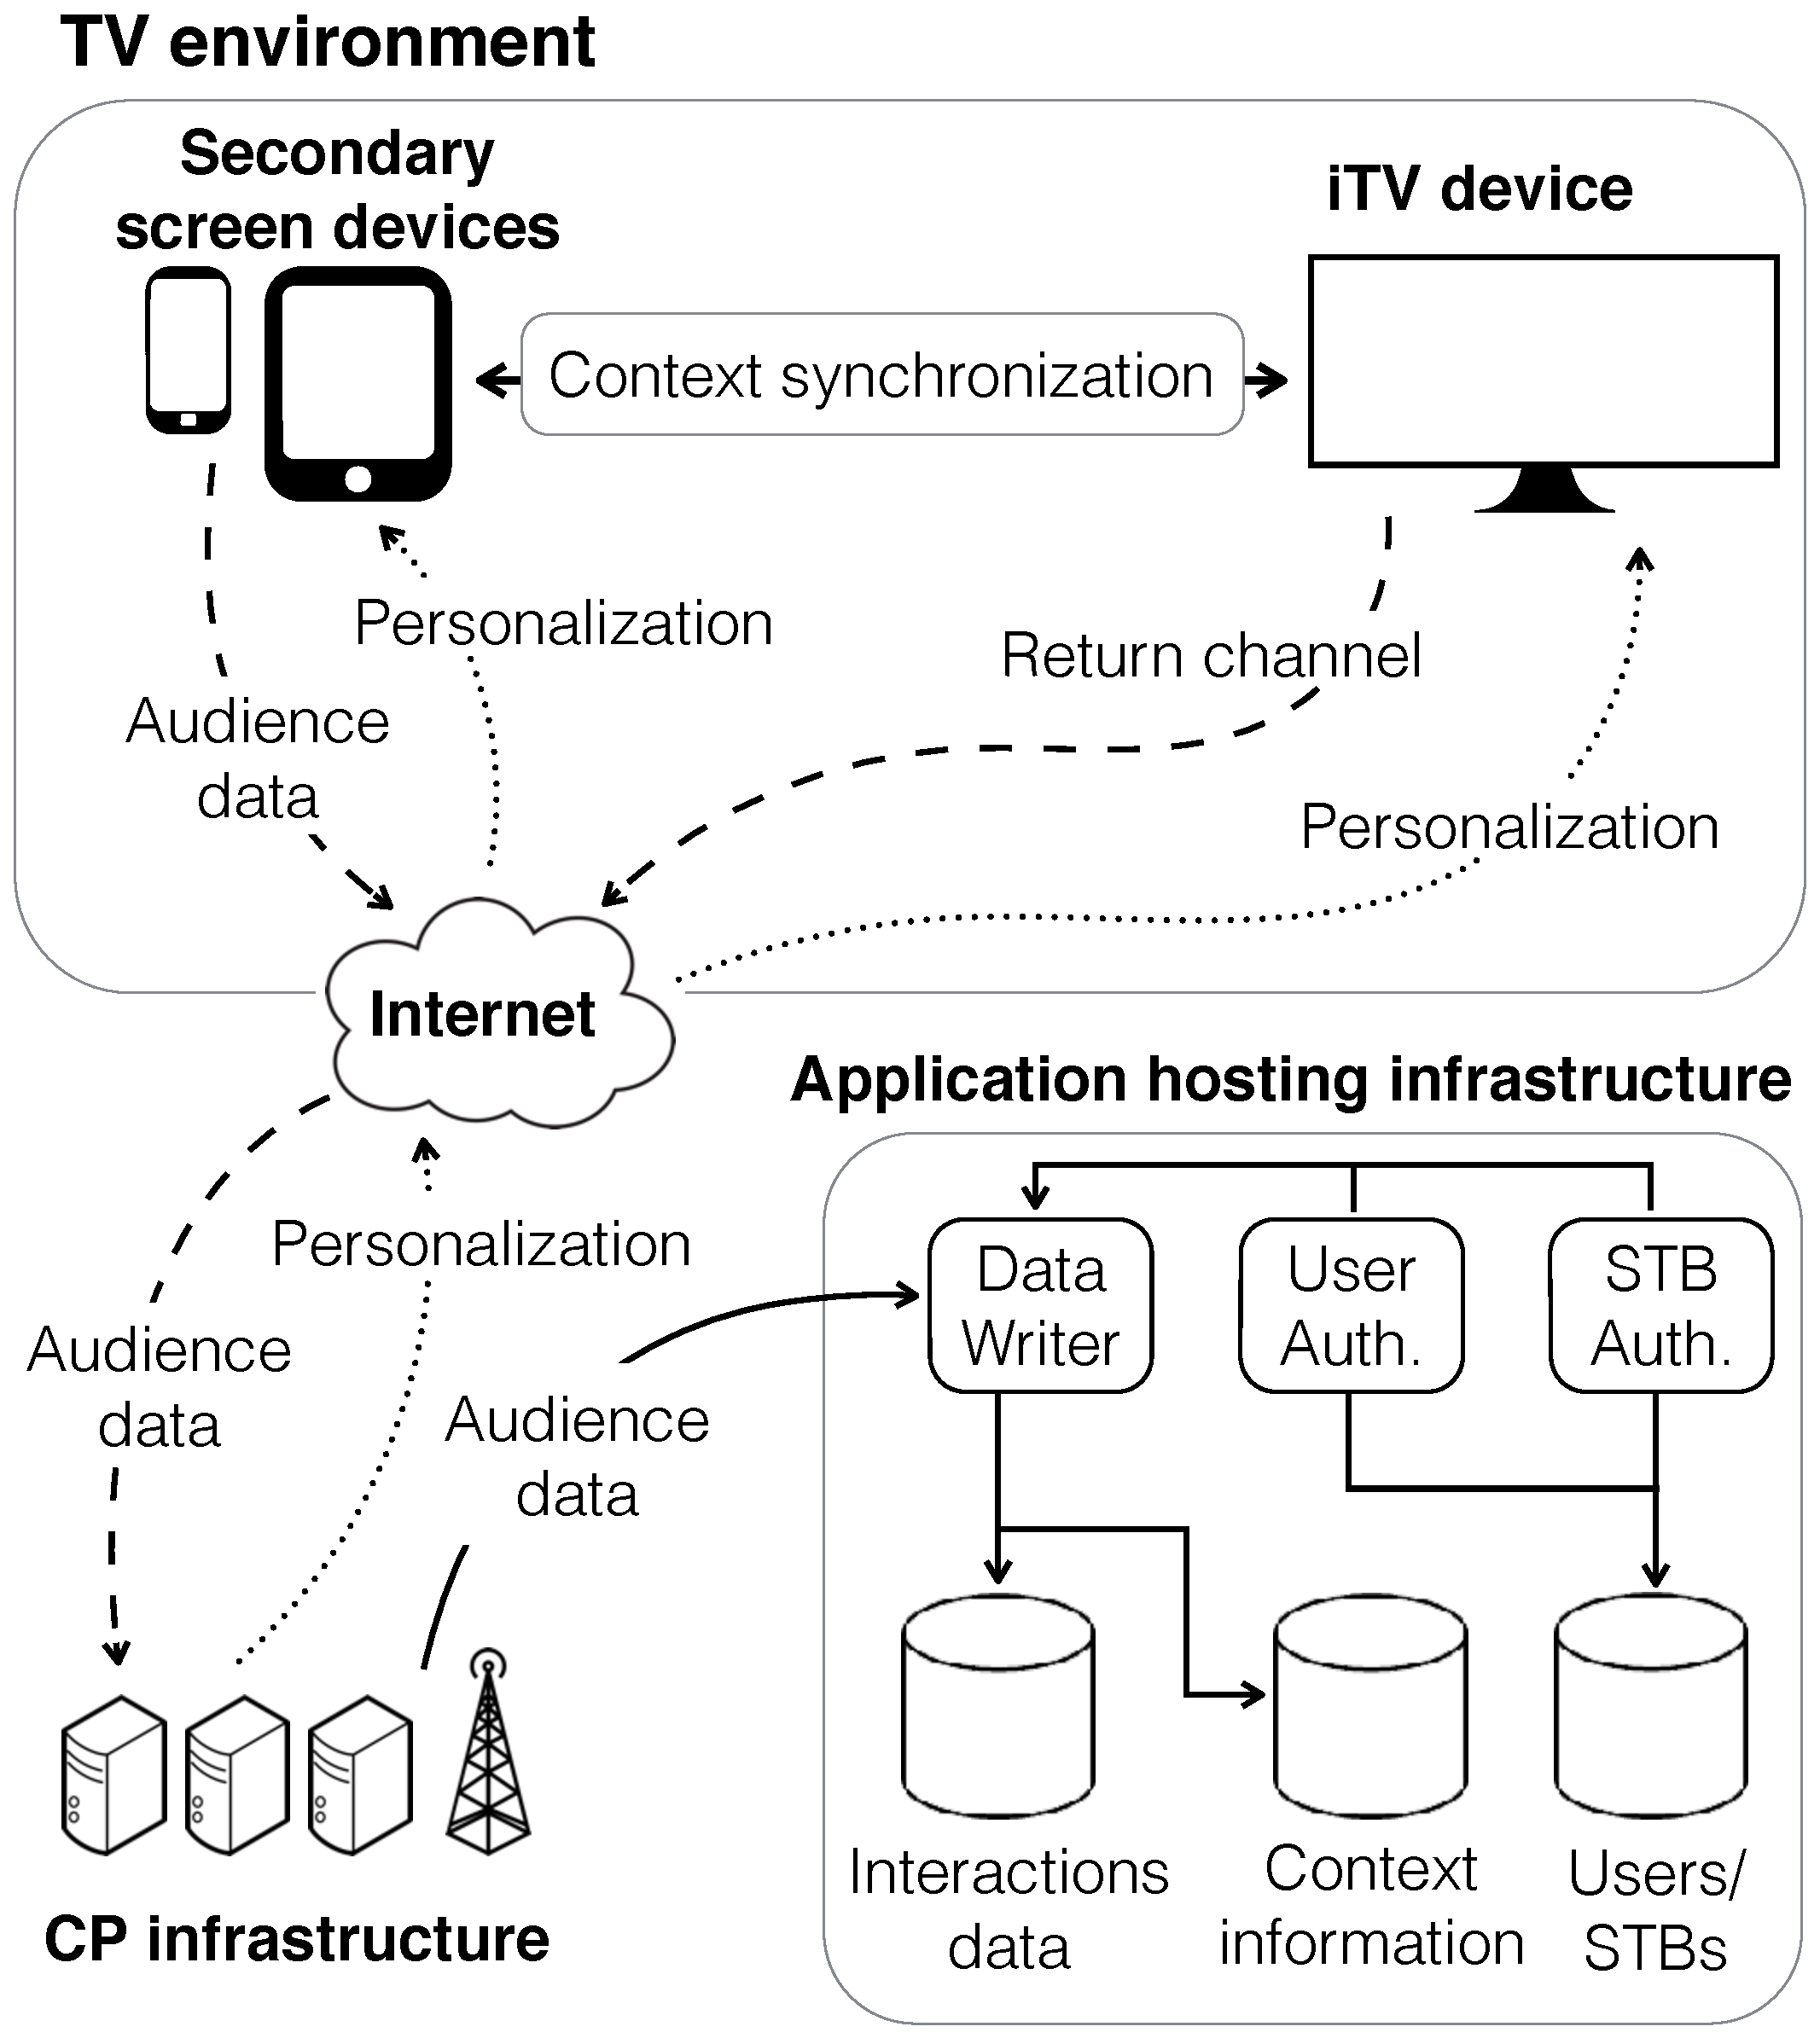
\includegraphics[width=3.5in]{img/architecture.pdf}
	\caption{Architecture to capture audience data. The viewers' interactions and the contextual information are captured and stored in the CP infrastructure.}
	\label{fig_architecture}
\end{figure}

A presence service detects physically nearby secondary screen devices that have the services necessary to establish a communication with an iTV device. Modern commercial operating systems for personal devices enable service discovery by using peer-to-peer or WiFi communication. This feature is particularly appropriated for the TV environment, once the secondary screen device must be wirelessly linked up with the iTV device. The devices are synchronized in order to update the contextual data about the viewer profile and the amount of people using a secondary device in the room. This contextual data can be used to learn how a viewer behaves towards other viewers. For example, a viewer behaves in a particular way while watching TV alone and the same viewer behaves in a different way while watching in group.

Viewers can use their secondary screen device to interact with TV by evaluating, commenting, sharing, or even recommending TV content to other viewers. The data related to those actions are naturally provided by the viewers, as part of the interaction, when using interactive applications (developed by the CP) installed in their secondary screen devices. The interactions and the contextual data are represented by the audience data, which is sent to CP infrastructure through Internet. Then, a Data Writer service stores the audience data related to each particular viewer and the iTV device.

The Data Writer service in the application hosting infrastructure consists basically of web services that provide interoperability among secondary screen devices, iTV devices and the CP infrastructure. The main advantage of this approach is the independence of operating system and programming languages used in the personal devices.

Once the audience data is stored, the CP can use this data to derive valuable information about users' tastes. This information can be used to provide personalized content to viewers based on the current context. Thus, the personalized content can be delivered via Internet to the secondary screen device or even to the TV, depending on the context.

\subsection{Web Services Design}

- RESTful API

- Resources

\subsection{iTV Environment}

- set-top box

- Service discovery

- context synchronization

\subsection{Second Screen Devices}

\section{Secondary Screen Implementation}

\subsection{RESTful API}

\subsection{Web Service Consumption}

\subsection{iTV and Secondary Screen Devices Communication}

\section{Experiments}

\section{Conclusions}

The use of personal devices as secondary screens arises as a new trend in TV environments. This paper presents an architecture to accurately capture audience data by using secondary screen devices and iTV devices. This architecture take advantage of the ubiquity and interactive capabilities of secondary screen devices to identify viewers and provide feedback for CPs through viewers' interactions and contextual information. The captured data relates to a single viewer in a given context. By using proper machine learning algorithms, this data can provide valuable information about viewers. Knowing this information can be very useful for CPs to improve their services aiming to increase the audience and to enrich user experience. As an example, CPs can deliver personalized content for a single person as well as for groups of people by using content recommendation algorithms.

An implementation of the architecture that is described in this paper is under development in a commercial cloud computing platform, which plays the role of the application hosting infrastructure. A web application that consists of a content rating system was developed to store  viewers' evaluations toward audio visual content, and a secondary screen client is under development. Some RESTful web services were developed to provide interoperability among the secondary screen devices and the web application. Thus, the interactions that are captured during the use of the secondary screen application are sent to the CP by means of HTTP requests to RESTful web services. Although the secondary screen application is not fully finished yet, some specific features have been tested to capture viewers' interactions as they occur.

The architecture described in this paper is also technically feasible to implement in Digital TV (DTV) systems and can be particularly interesting for CPs in DTV standards, e.g., the Brazilian (ISDB-TB) and the Japanese(ISDB-T). These standards support the use of mobile devices as part of the system. Since the mobile devices support the implementation of the DTV middleware, a cooperative exhibition of the DTV application can be managed with the iTV device, thus enabling the capture of viewers' interactions and contextual data.

\bibliographystyle{IEEEtran}
\bibliography{biblio}

\end{document}